\documentclass[10pt]{article}
\usepackage{graphicx,amssymb, amstext, amsmath, epstopdf, booktabs, 
verbatim, gensymb, geometry, appendix, natbib, lmodern, hyperref, float, titlesec, subfig}
\geometry{letterpaper}
%\usepackage{garamond}

\newcommand*\Title{Neurowrx Account Manual}
\newcommand*\cpiType{some subtitle}
\newcommand*\Date{Novermber 2018}
\newcommand*\Author{Michael Braeutigam}
\title{Neurowrx Account Manual}
\author{Michael Braeutigam}
\date{\today}
%-----------------------------------------------------------

\usepackage{cpistuff/cpi} % This is what makes your document look like a cpi document.


\begin{document}

\begin{titlepage}
\maketitle
\end{titlepage}

\linespread{1.15} %Set standard document linespacing

\begin{executive}

This is a document describing the fuctionality of the neurowrx website.

\frame{
\textbf{Important Title}

This is a convenient place to put any necessary legal mumbo-jumbo}
\end{executive}

\tableofcontents









%\subsection{green writing}

%Use the \texttt{callout} command:

%\callout{By the shores of gitchee gumee\\ by the shining big sea waters \\ stood the wigwam of Nokomis \\ brother of the moon, Nokomis.}



%Use the \texttt{frame} command:

%\frame{ 'Twas brillig and the slithy toves did gyre and gimble in the wabe \\ all mimsy were the borogroves, and the mome raths outgrabe. \\ Beware the Jabberwock, my son, the claws that bite, the jaws that snatch \\ Beware the Jubjub bird, and shun the frumious Bandersnatch.}

%\ref{accountemail} returns the index of the figure in the document


\section{Ordinary Members}

\subsection{Account Creation}

\begin{flushleft}
Once you are a neurowrx member, a username (probably based on your actual name, or organization name) will be chosen by the site admin, and you will receive an email at the address that you provided in your application.  It will have neurowrx in the subject line so check your spam filter if you do not receive it promptly.  It will notify you of your username and give you a link to a page where you can set your password, as well as a link to the regular login panel.  The login panel can be reached though this link or though the main site at \url{https://neurowrx.org/}, by clicking on the button at the top right corner. 
\end{flushleft}

\begin{figure}[h]
\centering
\caption{A typical account creation email}
\label{accountemail}
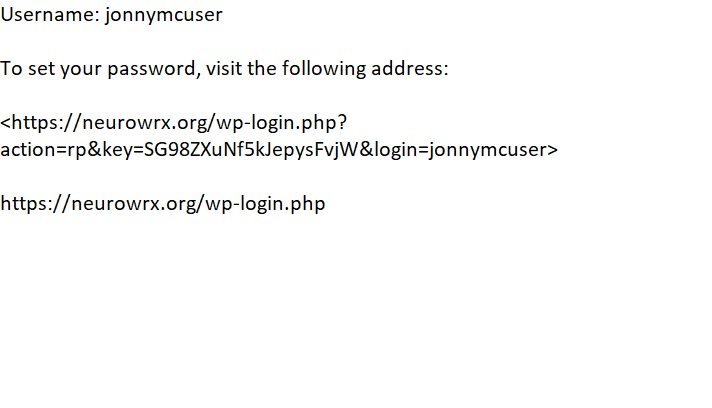
\includegraphics[scale=1.0]{images/accountcreation.jpg}
\end{figure}

The account's password is initially randomized and should be set via the first link before one attempts to log in.  In the case that the password is forgotten, it can be recovered though a link on the main login page at \url{https://neurowrx.org/wp-login.php}.

\begin{figure}[h]
    \centering
    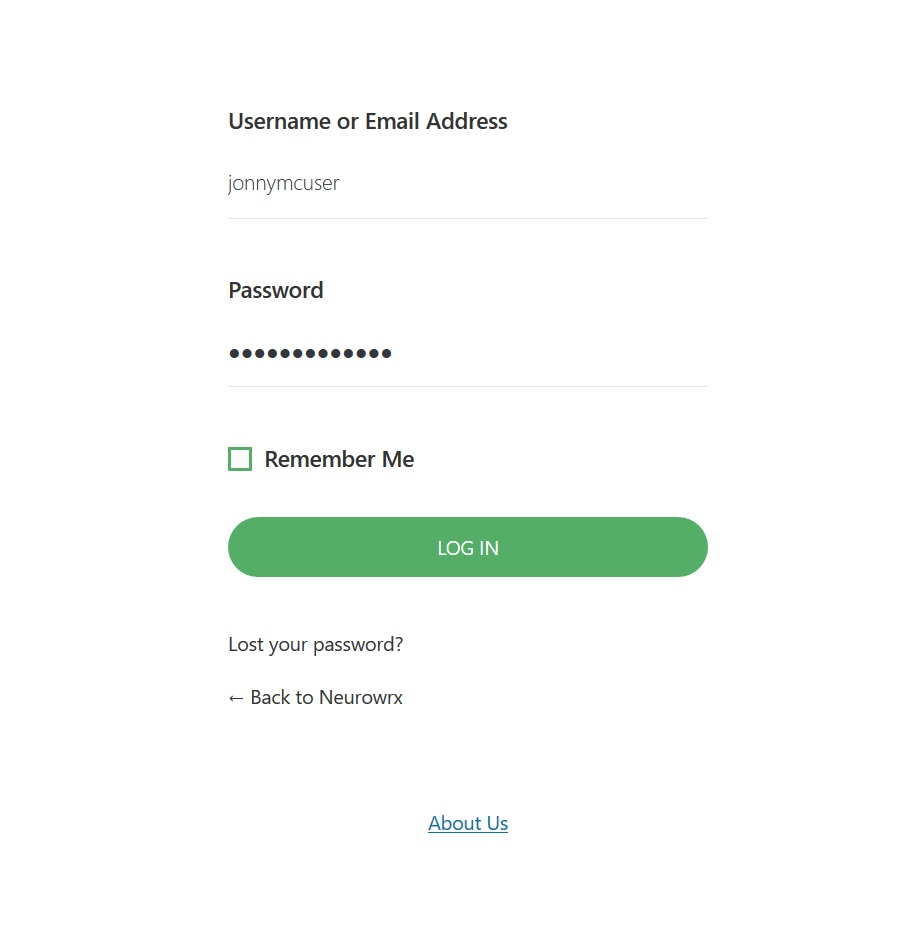
\includegraphics[scale=0.3]{images/loginpage.jpg}
    \caption{The login page}
    \label{loginpage}
\end{figure}

\begin{flushleft}
After you have chosen your password, you can log in with either your username, or with your email address.  Both are required to be unique, and in the case that you have more than one account; you must provide distinct email addresses for distinct accounts. 
\end{flushleft}

\begin{flushleft}
Once a successful login has occurred, the top panel of the website changes to give the user access to the communication features.  A link for the members section appears, as well as an icon for private messages, notifications, and another for settings.  There is also a menu hiding under the profile picture with more features which will be discussed in succeeding sections. 
\end{flushleft}

\begin{figure}[h]
    \centering
    
\includegraphics[scale=0.3]{images/topbar.jpg}
    \caption{The top panel that is publicly visible}
    \label{topbar}
\end{figure}

\begin{figure}[h]
    \centering
    
\includegraphics[scale=0.3]{images/topbarlogged.jpg}
    \caption{The top panel after login}
    \label{topbarlogged}
\end{figure}

\subsection{Your Neurowrx profile}

\begin{flushleft}
By hovering the mouse over the profile pic, a dropdown menu (with association submenus) becomes available.  The profile functions can either be accessed though the profile submenu or by clicking on "profile" itself to go to the profile page.  
\end{flushleft}

\begin{figure}[H]
    \centering
    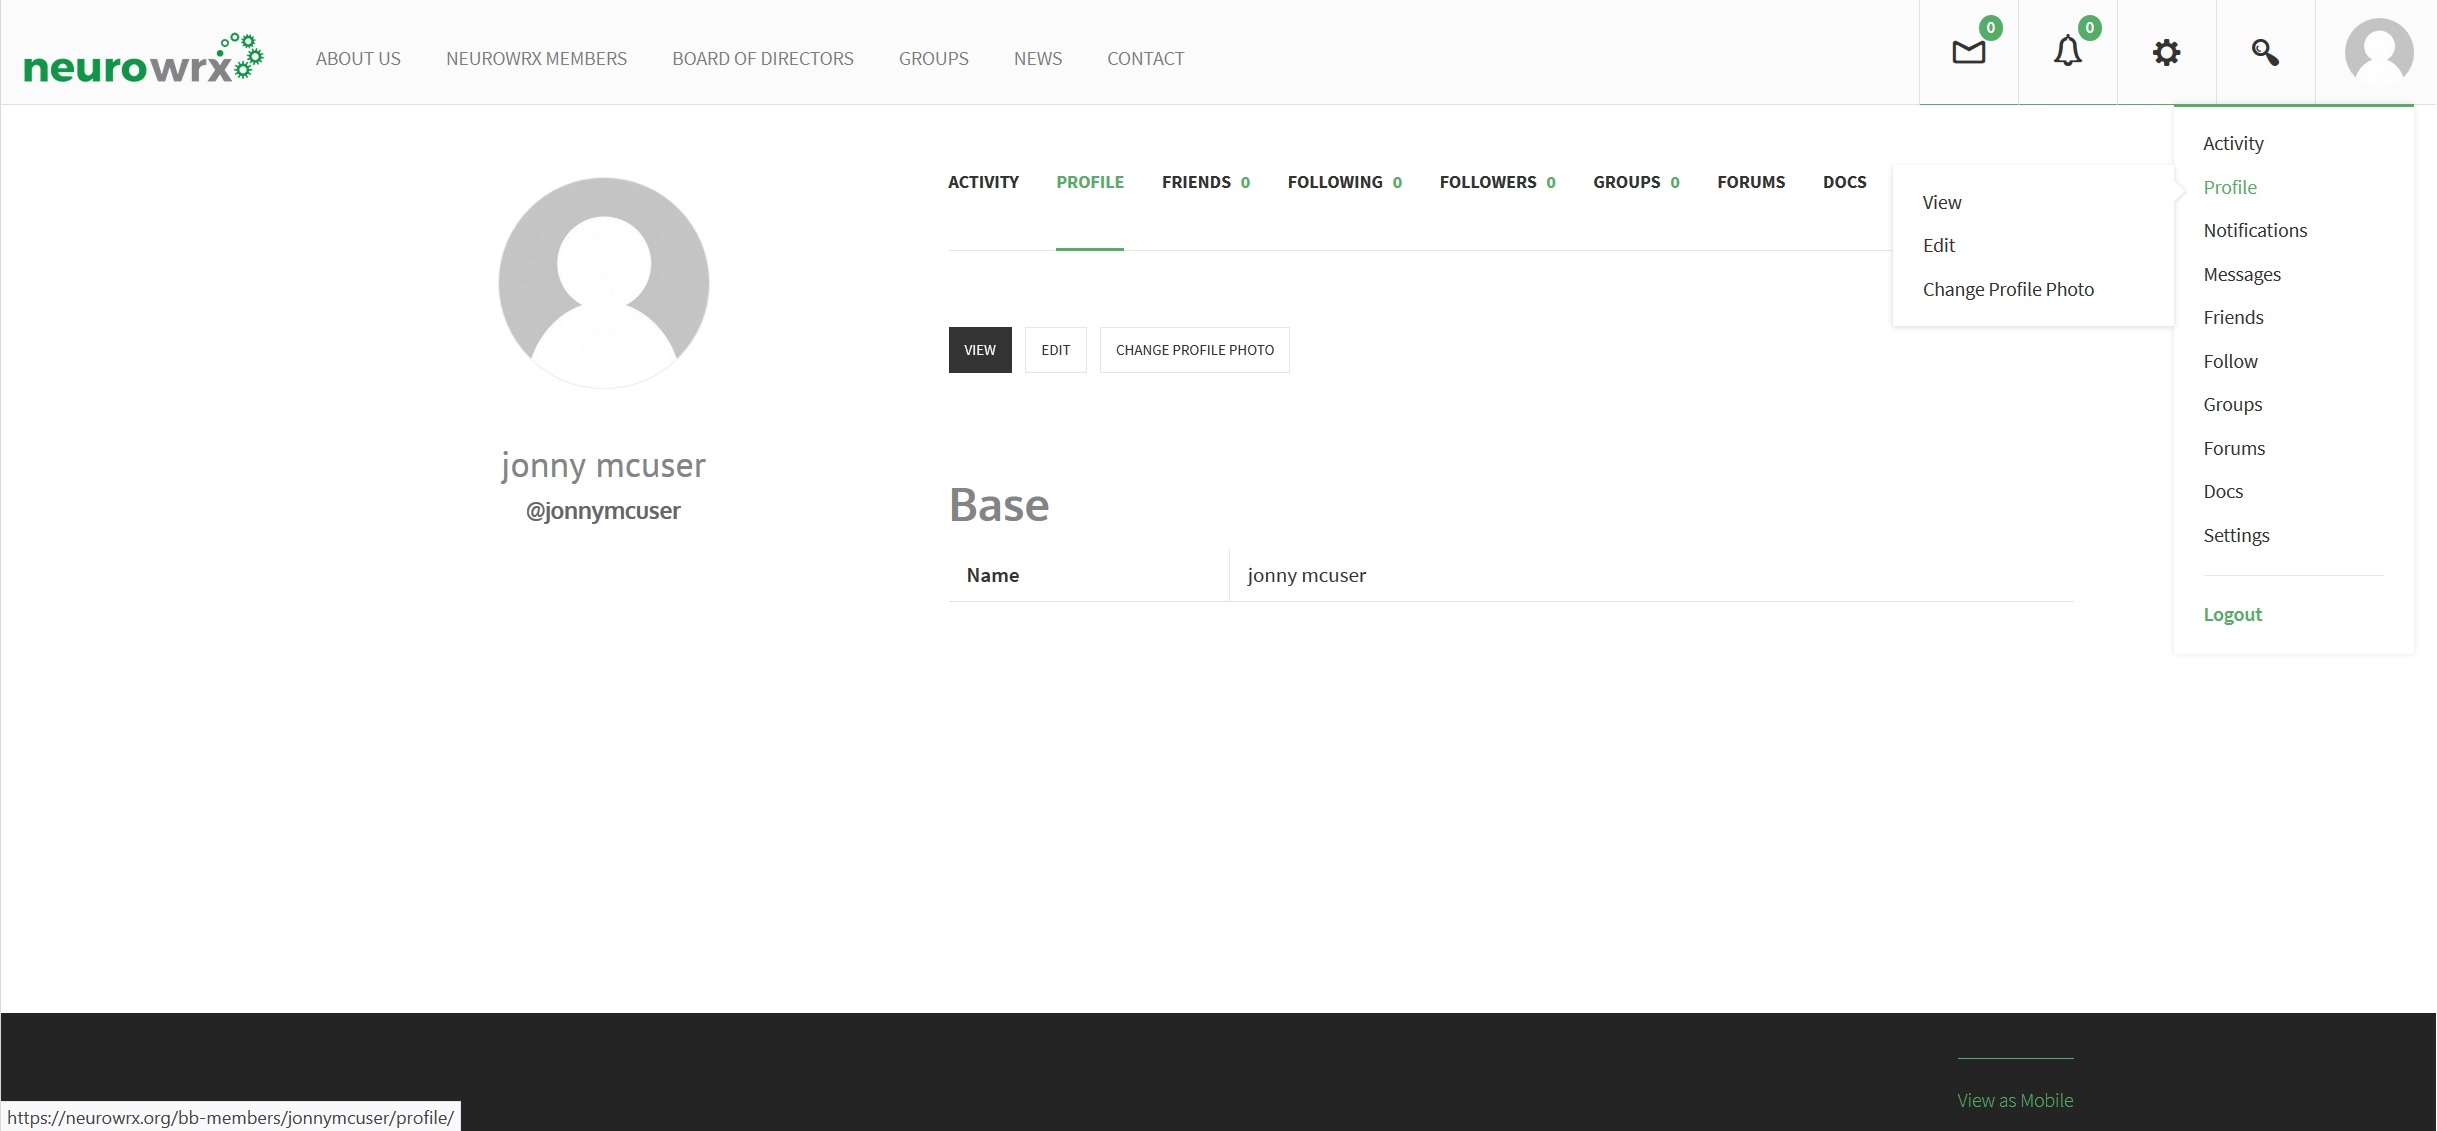
\includegraphics[scale=0.2]{images/profile.jpg}
    \caption{The profile page, and the profile menu that can be used to navigate to it.}
    \label{profilepage}
\end{figure}

\subsubsection{Changing your profile picture}

\begin{flushleft}
When you add a profile picture (which is optional), you can either upload an existing file by dragging the file into the hatched boundary box (which doesn't work on all operating systems), open a file selection window by clicking the green button, or click the "Take Photo" link to activate your webcam (assuming that you have one plugged in).  This step makes the an image file available to the cropping tool, which you will use to select a small square shaped section of the image (presumably your face) for use as your face on the forums and in the messaging system. 

\end{flushleft}
 The image is required to be of the .jpeg, .gif, or .png file formats.  It is also recommended that you use an image that is of at least 280x280 pixels, but this isn't strictly necessary. 
\begin{flushleft}

\end{flushleft}

\begin{figure}[h]
    \centering
    \subfloat{{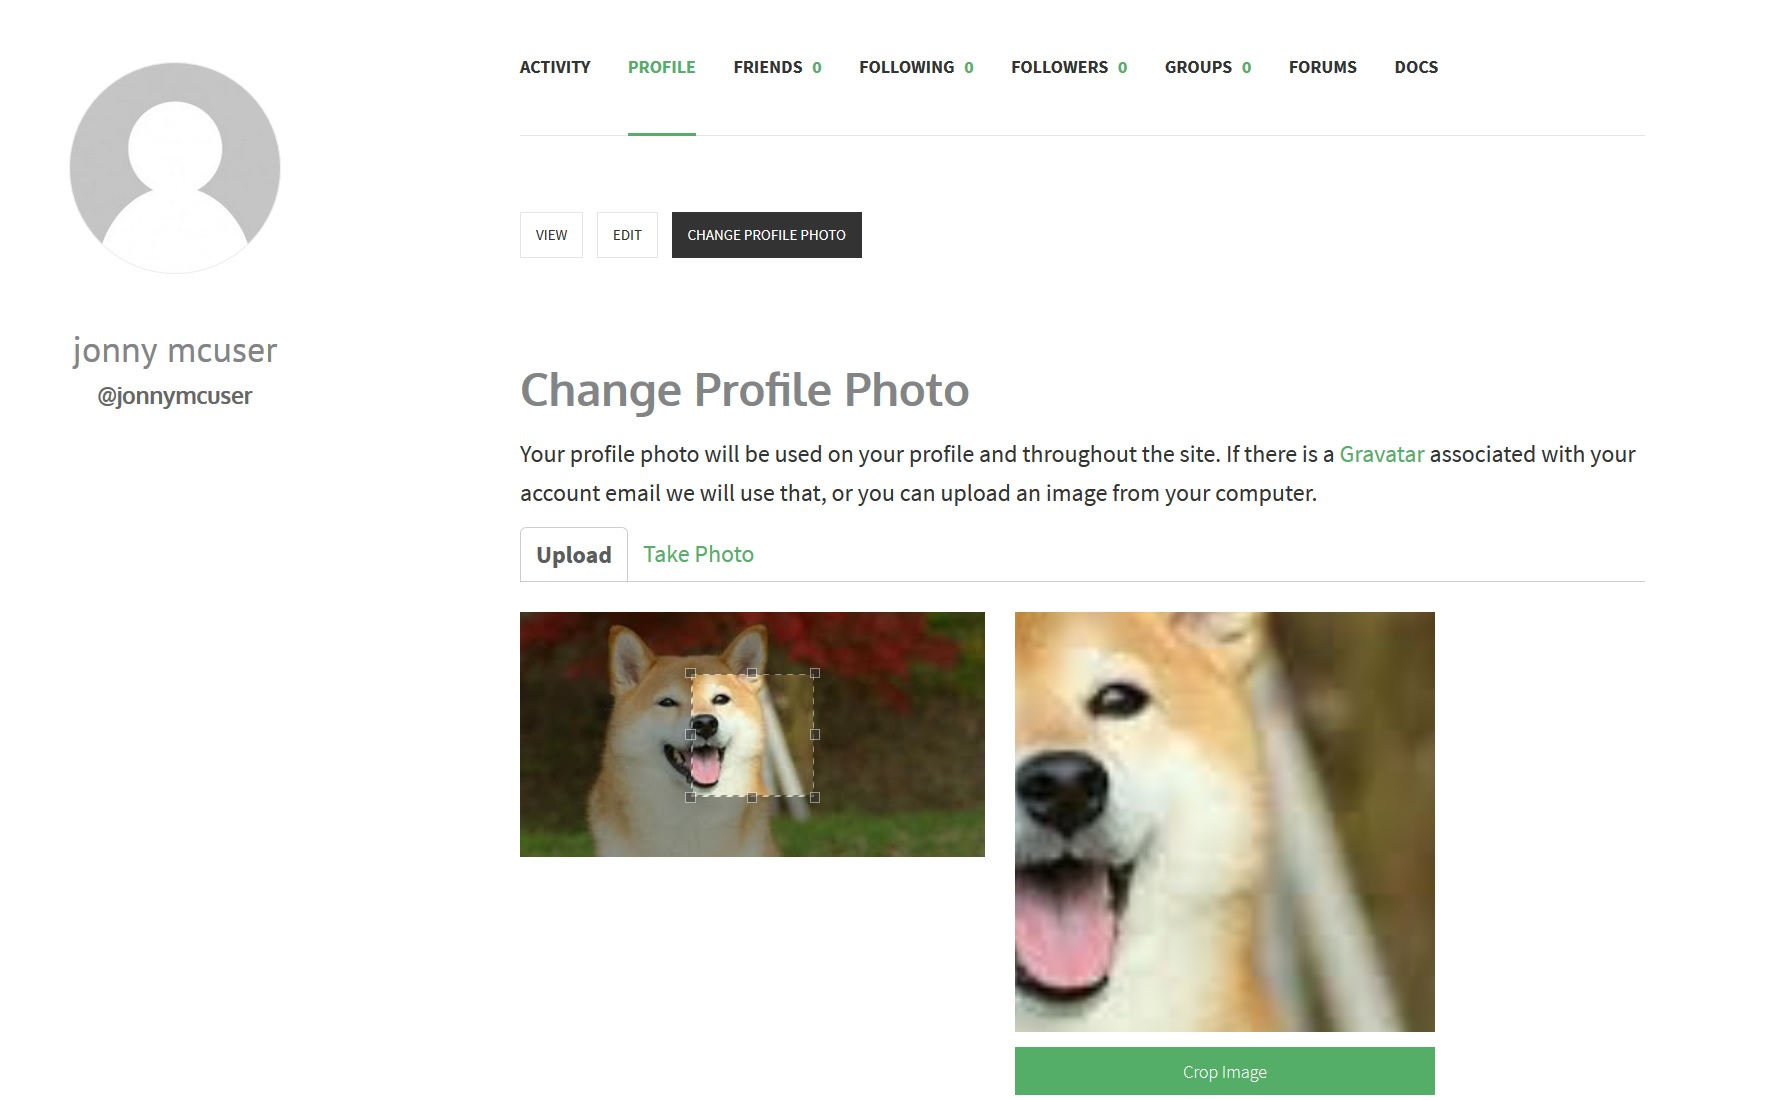
\includegraphics[scale=0.2]{images/doggy.jpg}}}
    \qquad
    \subfloat{{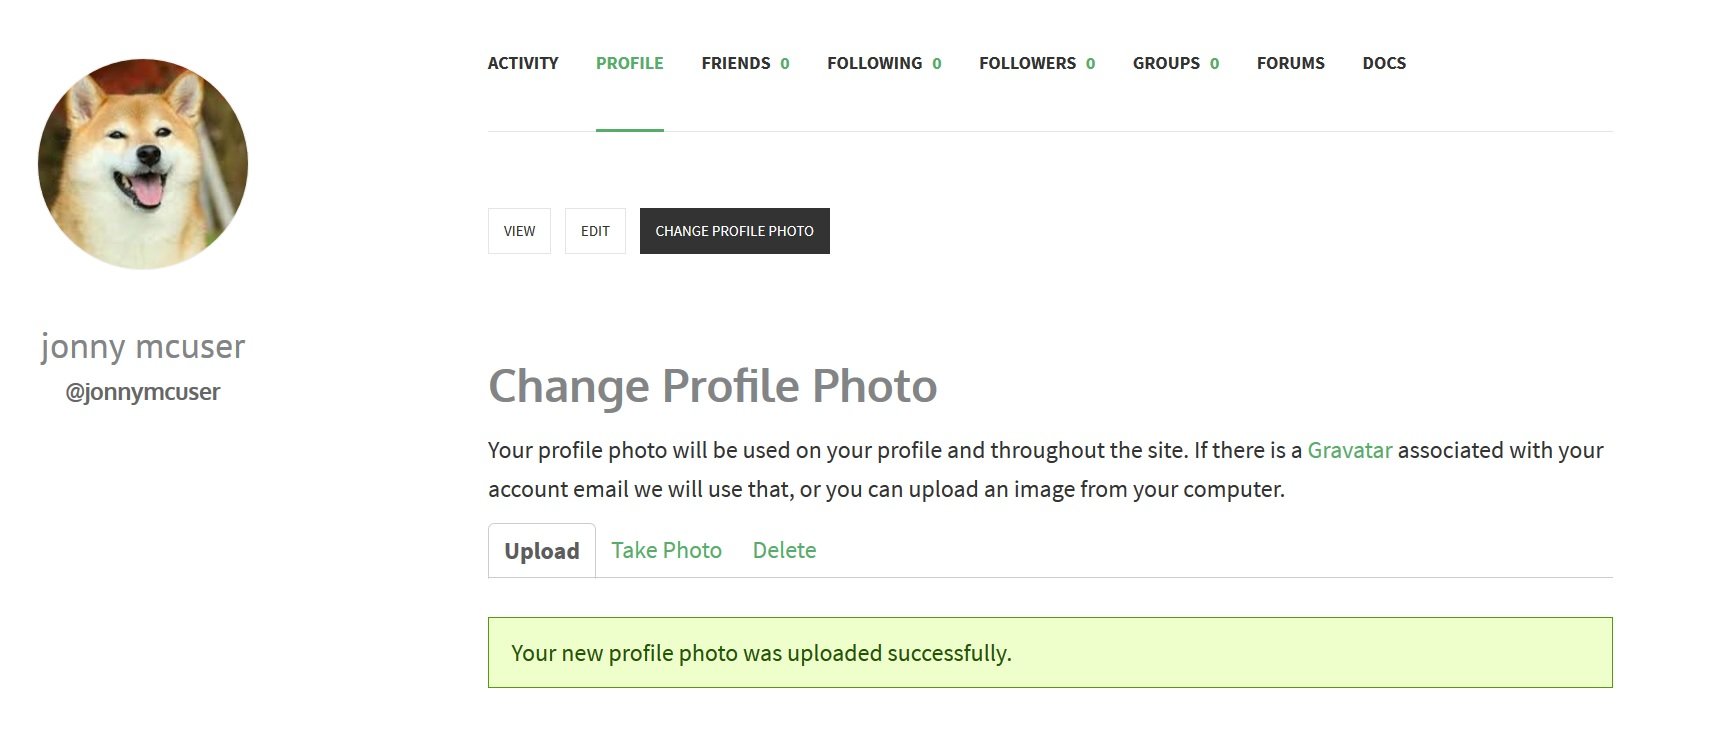
\includegraphics[scale=0.2]{images/doggy2.jpg}}}
    \caption{A successful profile picture upload}
    \label{avatarUp}
\end{figure}

\subsubsection{Editing your other profile information}

\begin{flushleft}
Other than the photo, your Neurowrx profile contains a changeable public Name field (which is not the same as your username) a gender field (which by default has neither selected, and does not have to be chosen) and several fields that you can paste links to your profiles on other social networking services.  At the time of this writing, we have fields for facebook, twitter and a few others.  This list could potentially grow in the future.  
\end{flushleft}

\begin{flushleft}
One is only expected to post the url of the profile in question, the form of which varies from service to service.  If you are unsure what the url to your profile is, consult the documentation for that particular service. 
\end{flushleft}


\subsection{Groups}
\begin{flushleft}
Most of the activity on this website occurs within the many groups that members can be part of.  They provide a forum for discussing relevant subject and sharing and editing documents.  There are two main pages where someone can interact with the group functions.  One can be reached by clicking on the "Groups" link located between the board of directors and news links on the top panel of the site.  This page lists all the groups on the site, and is where you request memberships to groups that you are not already a member of. 
\end{flushleft}

\begin{flushleft}
The other is located in the menu that arises from hovering the mouse over your profile picture. This section only lists groups that you are currently a member of.  It is also where you can accept invitations to groups that have been extended to you by their administrators. 
\end{flushleft}

\begin{figure}[h]
    \centering
    \subfloat{{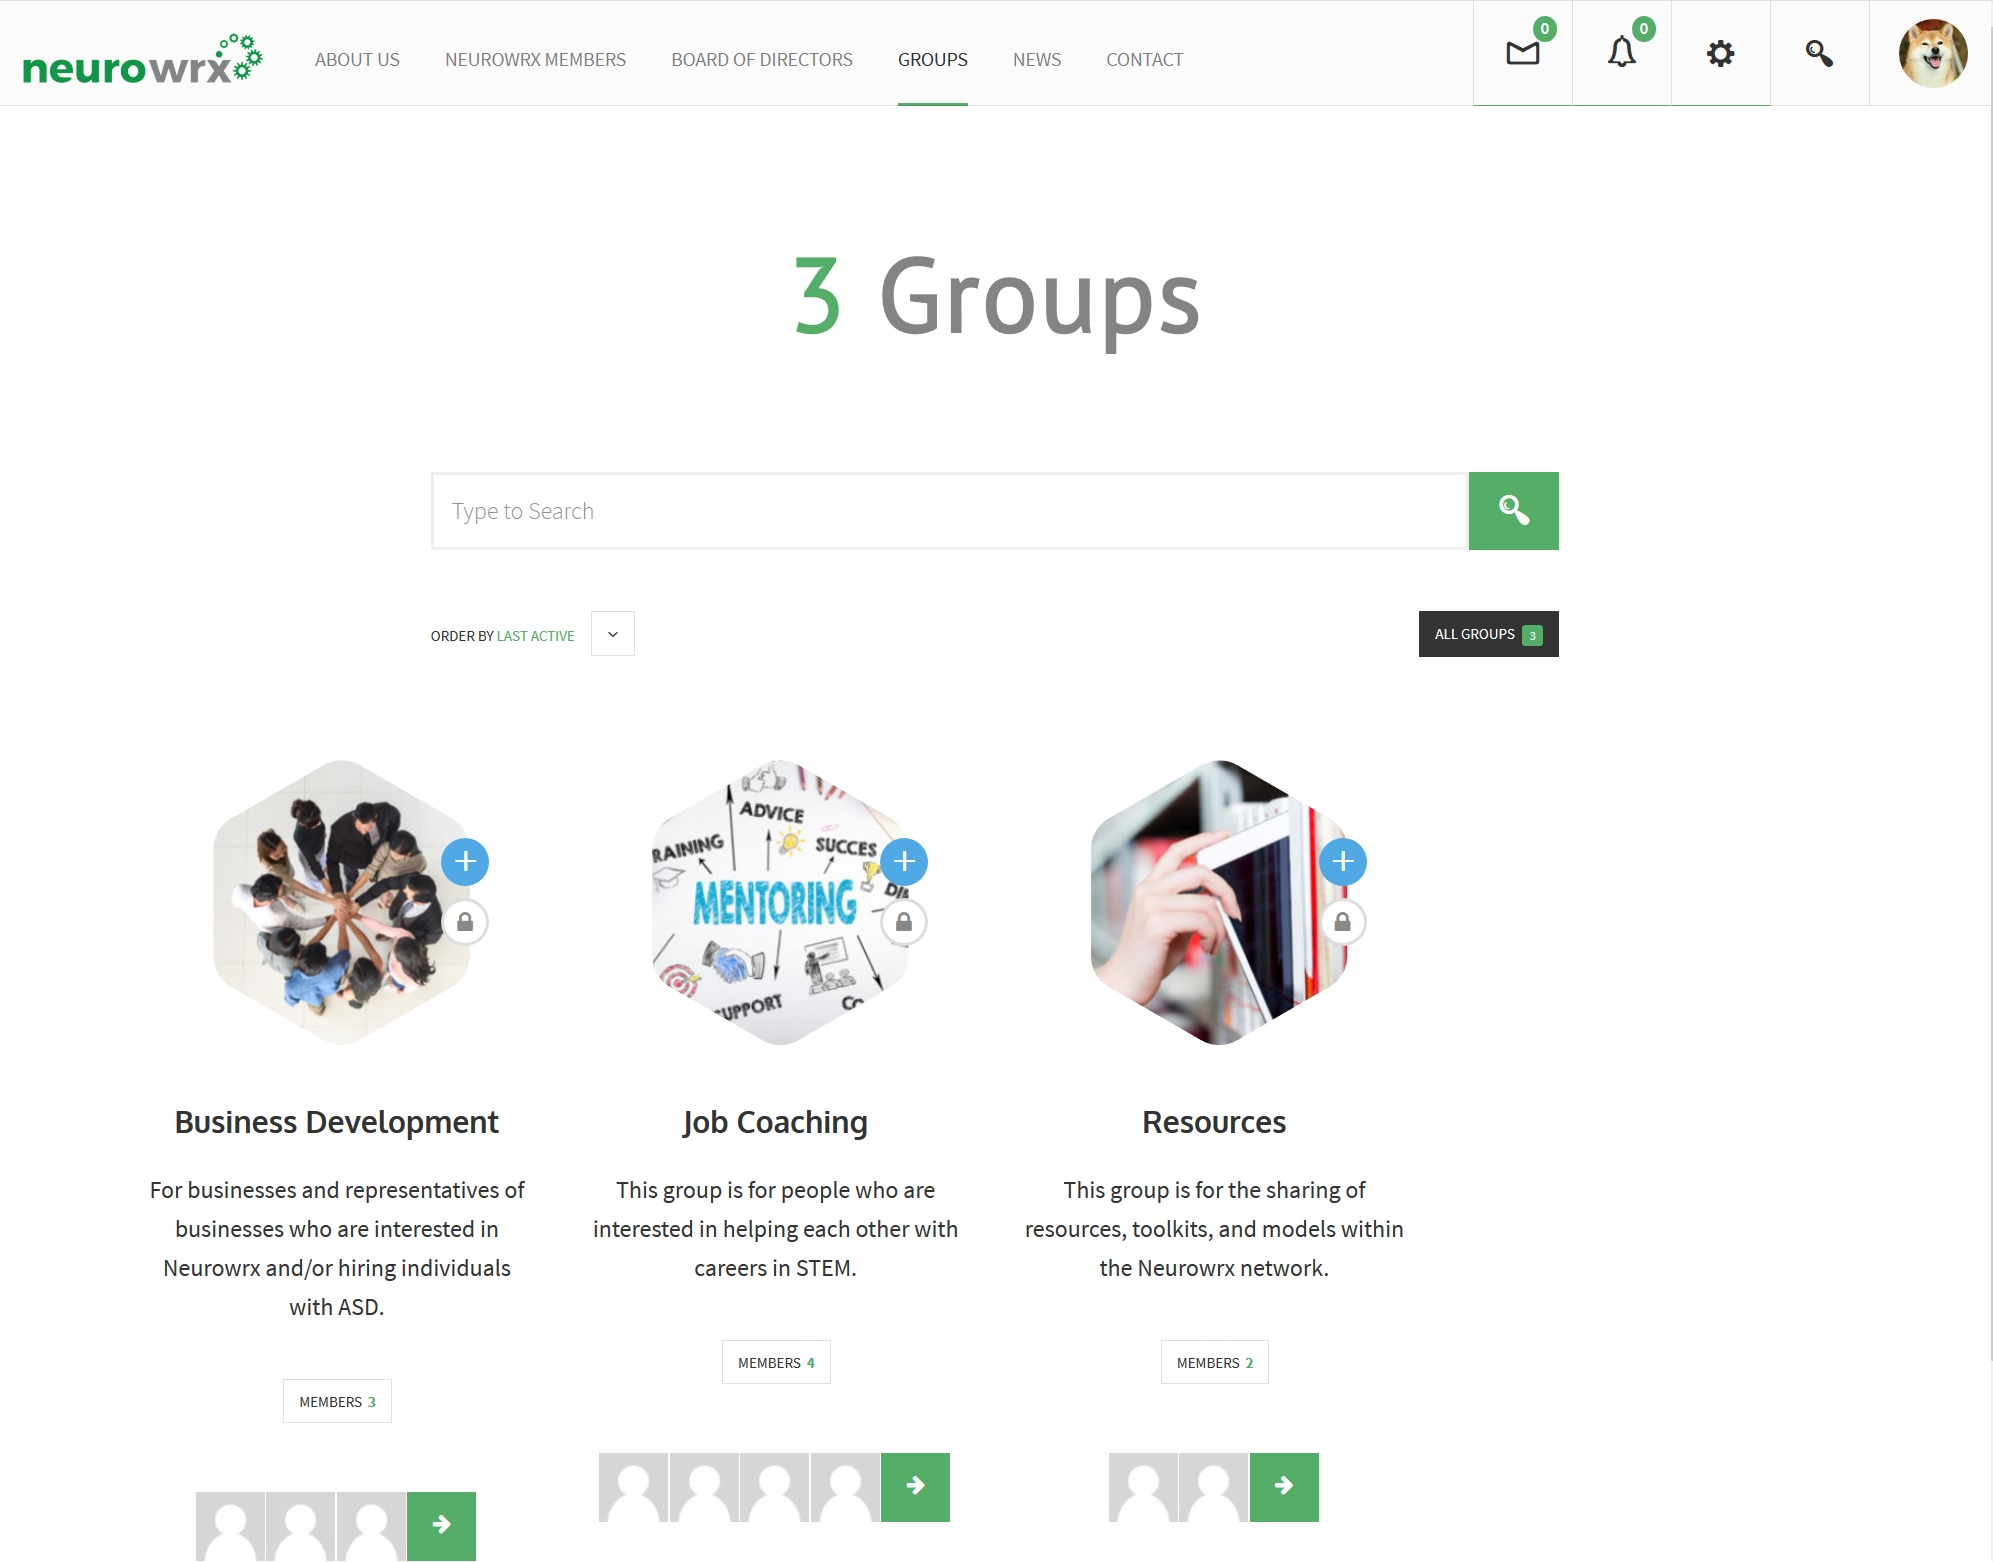
\includegraphics[scale=0.15]{images/allgroups.jpg}}}
    \qquad
    \subfloat{{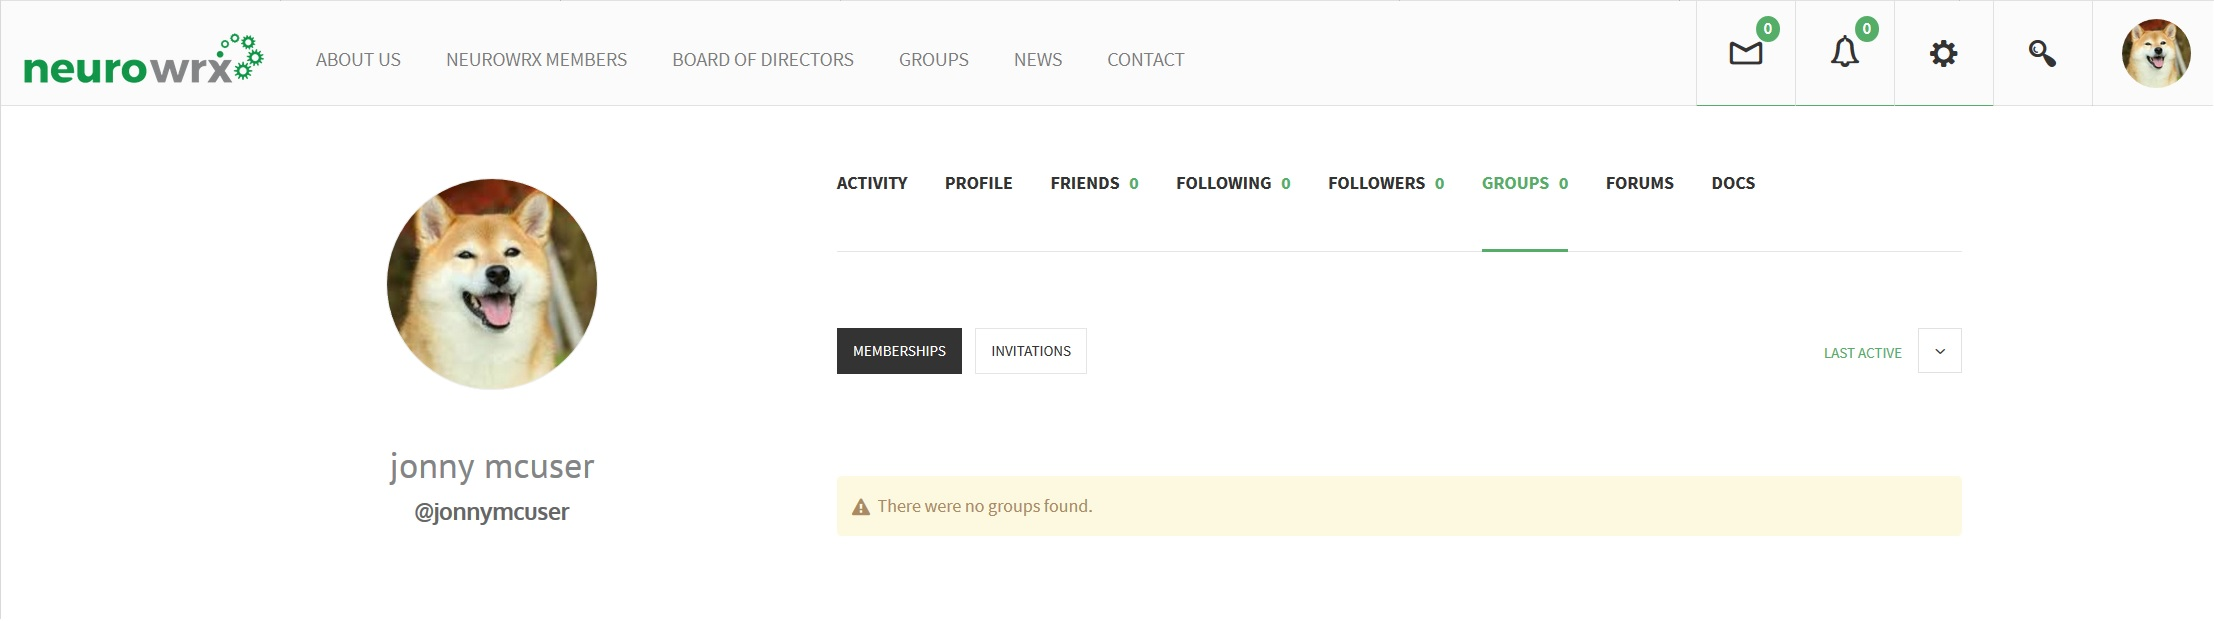
\includegraphics[scale=0.2]{images/usergroups.jpg}}}
    \caption{The general groups page accessed from the top panel (left) and the user's group page accessed though the dropdown menu (right)}
    \label{groupmenus}
\end{figure}

\subsubsection{Joining Groups}

\begin{flushleft}
To view the documents or discussions in a group, you must first be a member.  There are two ways to become a member of a group.  The first is that are invited by the group moderator, in which case the invite will be visible in the menu on the right in figure \ref{groupmenus}.  The second is that you apply for membership and your application is accepted by a group moderator.  This application is sent by clicking the plus sign in the blue circle to the upper right of the group avatar in the menu seen on the left in figure \ref{groupmenus}.  We will demonstrate both here. 
\end{flushleft}

\begin{flushleft}
When a request to join a particular group has been sent, by clicking on the send request button mentioned earlier, a red "x" appears in the upper right part of the plus symbol.  
\end{flushleft}

\begin{figure}[h]
    \centering
    
\includegraphics[scale=1]{images/requestsent.jpg}
    \caption{The request to join has been sent}
    \label{requestsent}
\end{figure}

\begin{flushleft}
One a forum moderator or administrator accepts your request, you will receive a notification that your membership has been accepted in your notifications panel. See figure \ref{youaremember}.
\end{flushleft}

\begin{figure}[h]
    \centering
    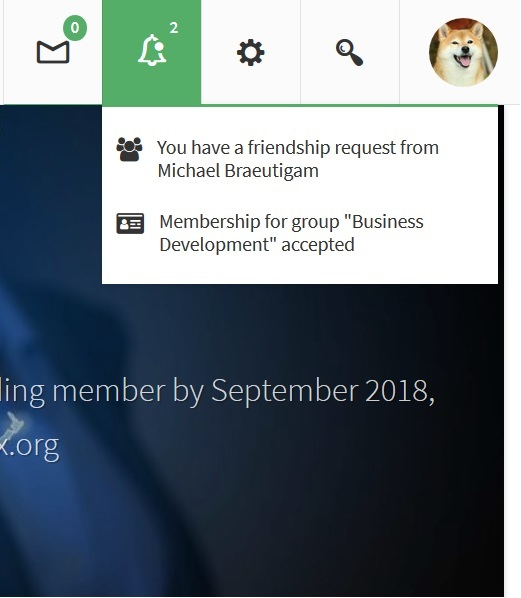
\includegraphics[scale=0.5]{images/youaremember.jpg}
    \caption{The member acceptance notification, at the bottom of the notification panel}
    \label{youaremember}
\end{figure}

\begin{flushleft}
The other way to end up a member of a group is for a current member who is your friend (see section \ref{Friendships}) to extend you an invitation, and for you to accept it.  When one of your friends sends you an invitation, it will appear in your notification panel.  You navigate to the page where an invitation can be accepted, you can either click the notification in the notification panel, or navigate to you personal groups page through the dropdown menu (see the right side of figure \ref{groupmenus}). 
\end{flushleft}

\begin{flushleft}
 In the second case, there is a button called "invitations" to the right of memberships that takes you to your pending invitations screen, which can either be accepted or rejected.  See figure \ref{invites}. 
\end{flushleft}

\begin{figure}[h]
    \centering
    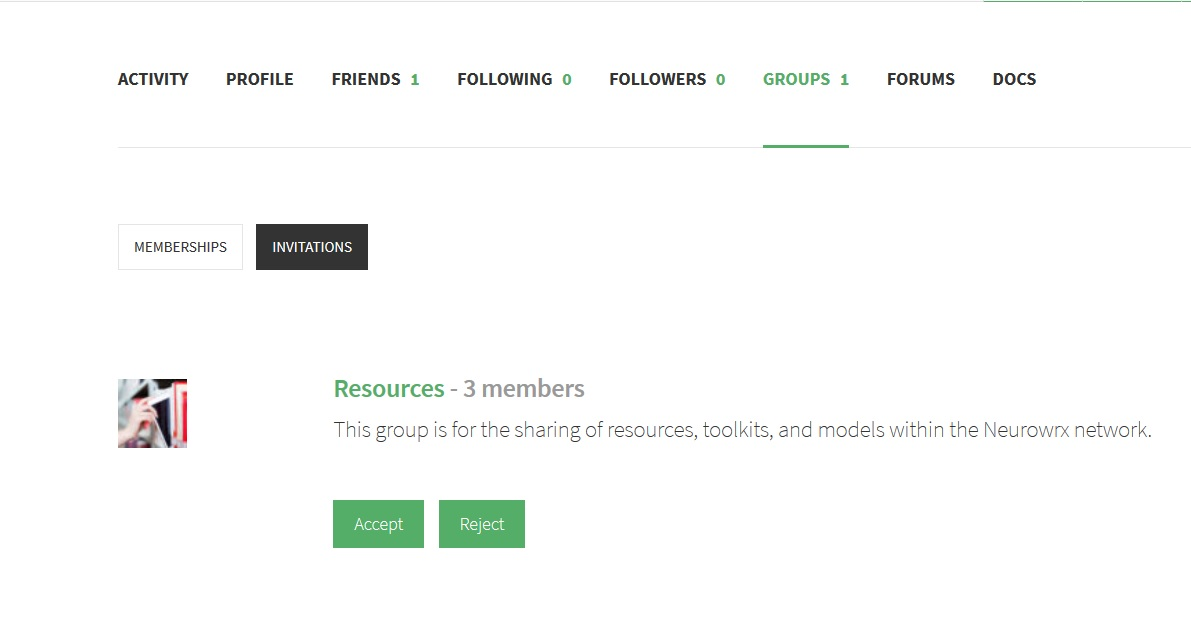
\includegraphics[scale=0.3]{images/invitations.jpg}
    \caption{Pending invitations screen}
    \label{invites}
\end{figure}

\subsubsection{Leaving Groups}

\begin{flushleft}
As with joining, there are multiple ways to leave a group.  The first is to go to the general groups page from the "Groups" link in the top panel (as in the left side of figure \ref{groupmenus}).  Once there, the groups that you are a member of (or have requested to be a member of) will have a red "x" at the top right of their blue "+" sign (see figure \ref{requestsent}).  If you click this icon, you membership to a group (or your request for membership) can be canceled, after confirmation. 
\end{flushleft}

\begin{flushleft}
The second way of leaving a group is to follow the same process as above, but from your personal groups page that is reached though the dropdown menu, as in the right side of figure \ref{groupmenus}.
\end{flushleft}

\begin{flushleft}
The third way is to go to the groups page itself, from either of the two previously mentioned menus, and click the green "leave group" button on the left hand side of the screen.  It is located below the groups avatar. 
\end{flushleft}

\begin{figure}[h]
    \centering
    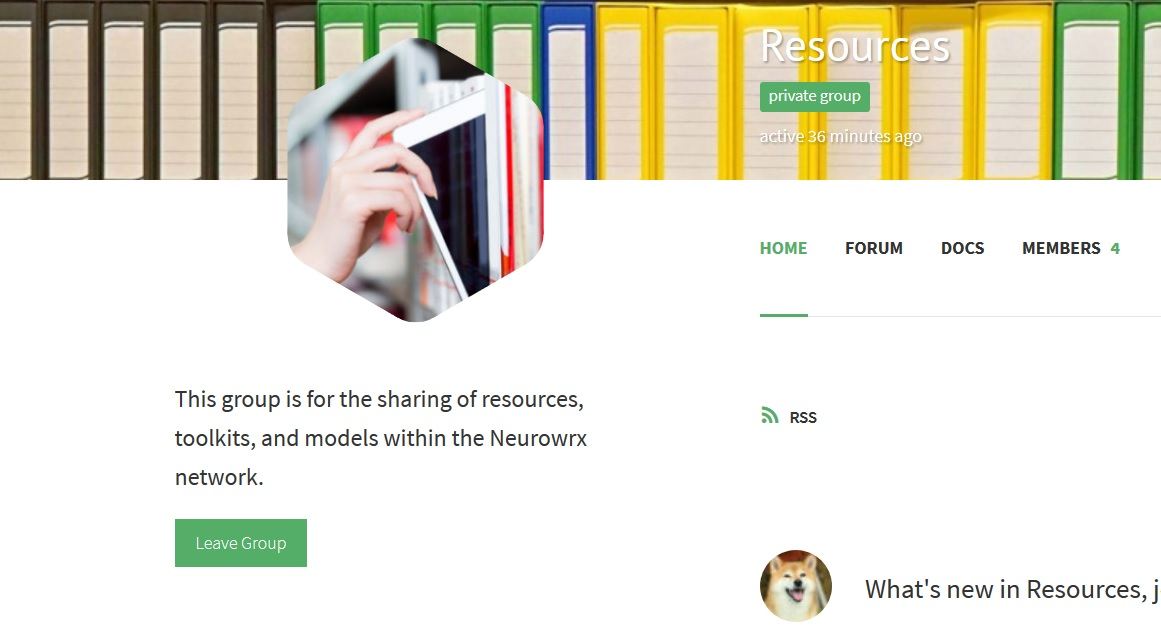
\includegraphics[scale=0.3]{images/leavegroup.jpg}
    \caption{The leave groups button on the groups main page}
    \label{leavegroup}
\end{figure}

\subsubsection{The forum associated with a group}
\subsubsection{The documents associated with a group}

\subsection{Friendships} \label{Friendships}
\subsection{Posts}
\subsection{Messages}

\section{Group Moderators}
Group moderators have elevated access and responsibilities.  They approve memberships for the groups assigned to them, and have the ability to remove content posted by uses, as well as remove users from groups.  The rules governing these things are a matter of policy and not defined in this document.  The following only covers how these things are to be achieved in the application itself. 

\subsection{Member Management}
\begin{flushleft}
Most of the membership management functions can be found in the manage section of a groups page, the link to which is only visible to either moderators or administrators.
\end{flushleft}

\begin{figure}[h]
    \centering
    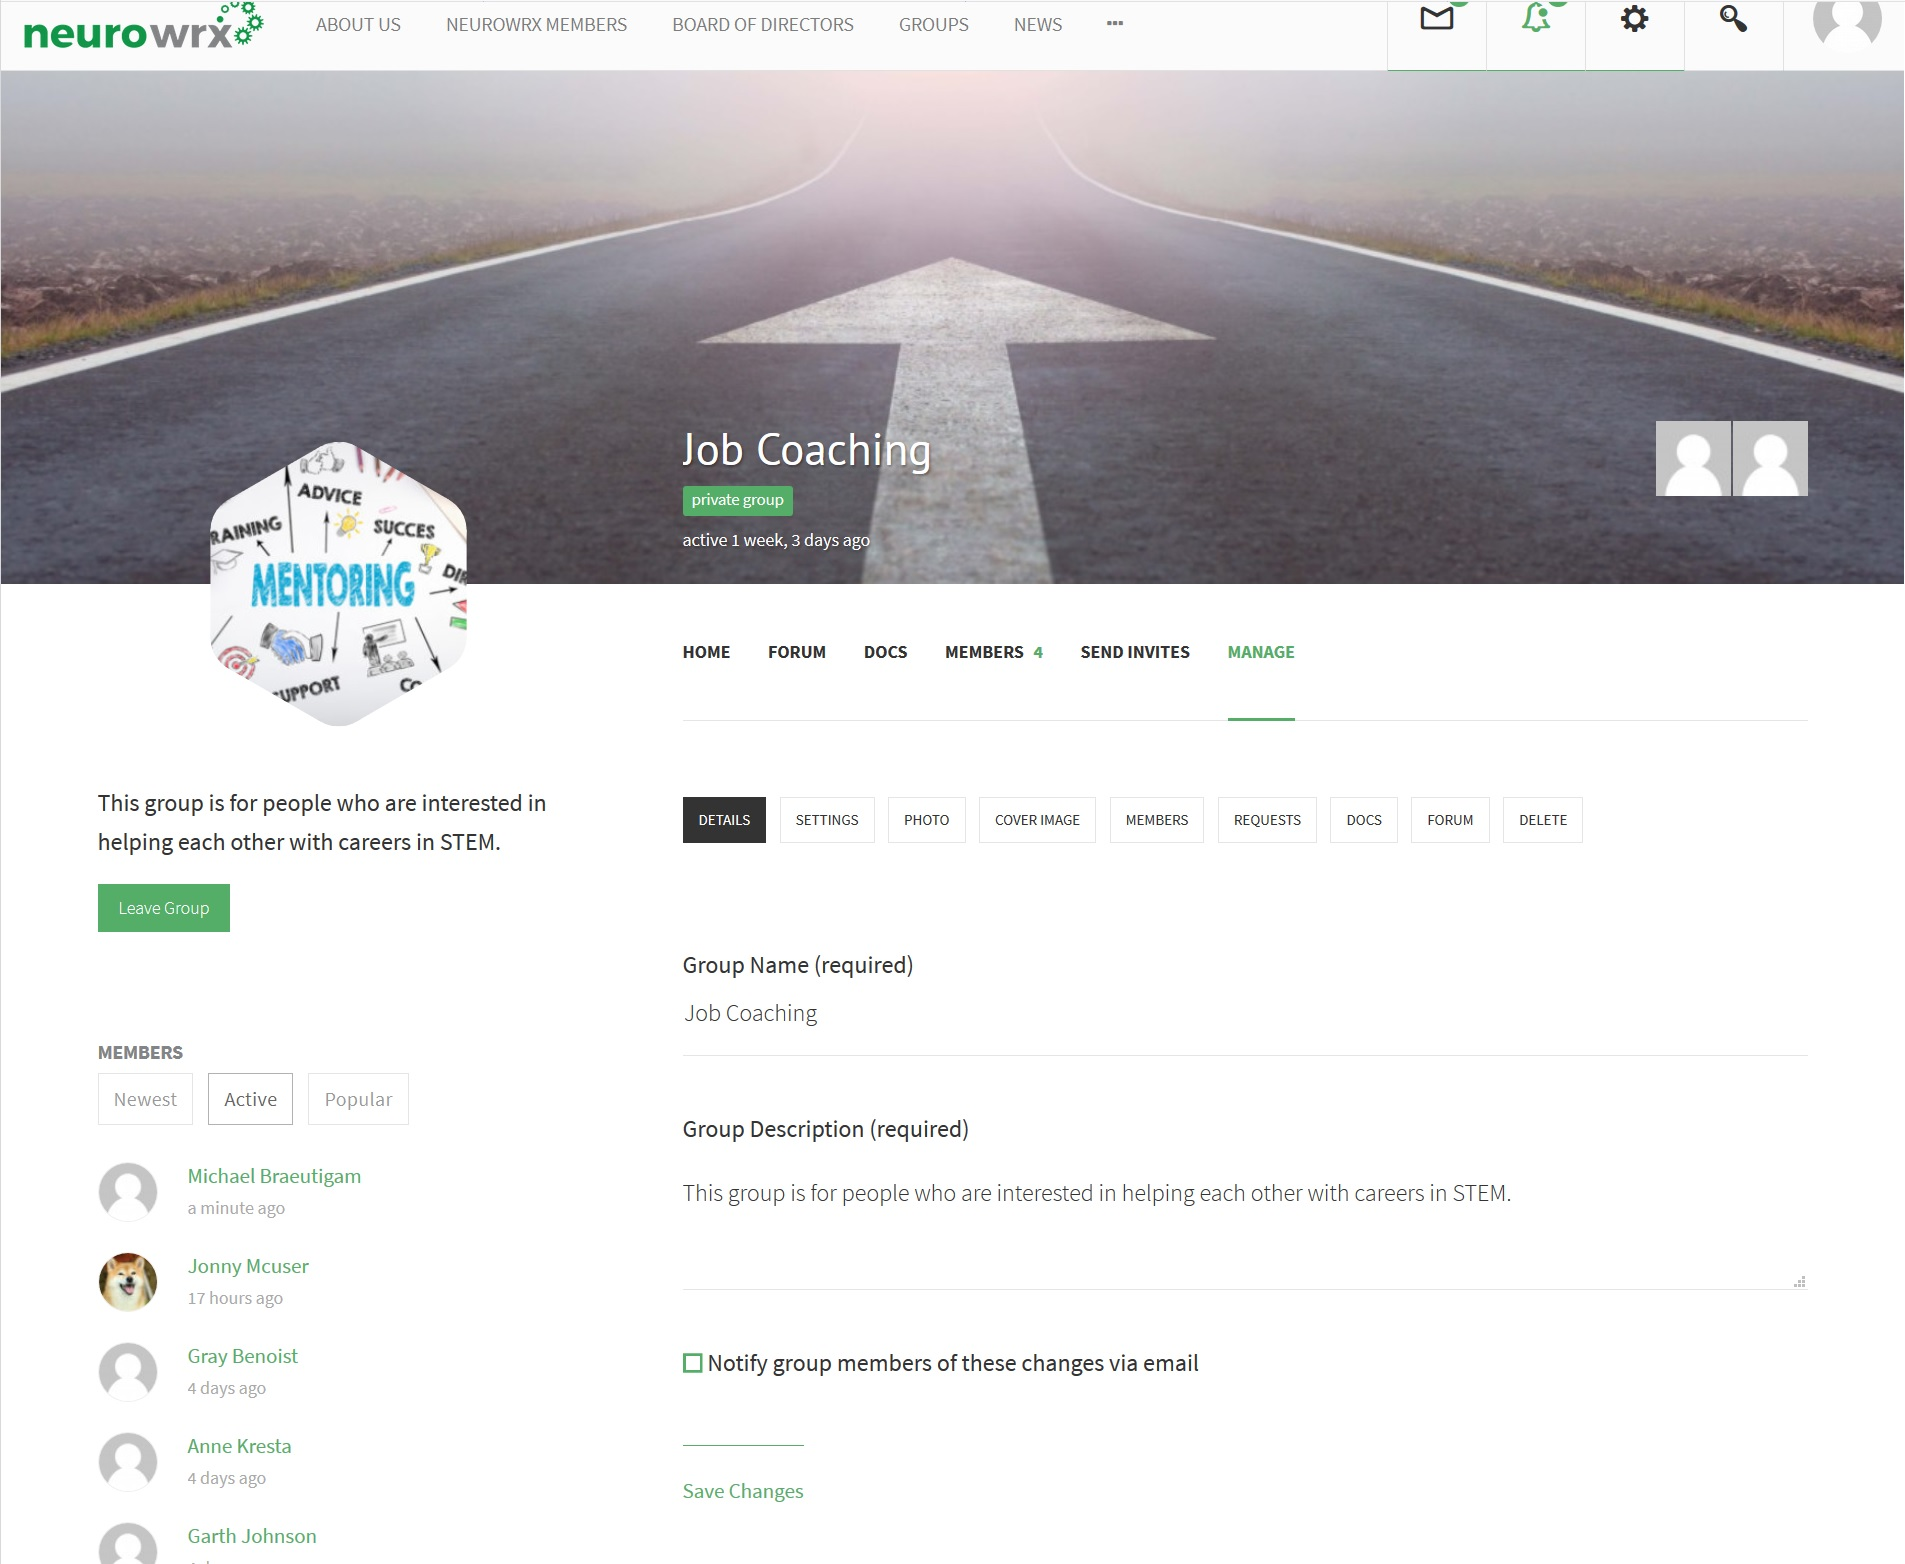
\includegraphics{images/groupmanage.jpg}
    \caption{The group management link is visible to moderators or adminstrators}
    \label{groupmanagelink}
\end{figure}

\subsubsection{Join Requests}

\begin{flushleft}
Join requests can be found in the requests submenu of the management section of a group. 
\end{flushleft}

\subsubsection{Removing Members}
\subsubsection{Promoting Members}
\subsection{Content Management}
\subsubsection{Posts}
\subsubsection{Documents}





\section{Administrators}
\bibliography{codes_impact}
\bibliographystyle{plainnat}
\end{document}